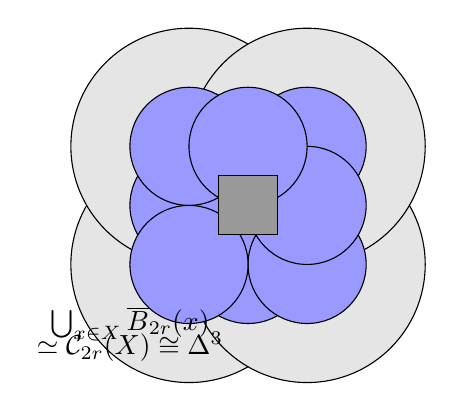
\begin{tikzpicture}[scale=1.5]
            % Draw circles
            \draw[fill=gray!20] (0,0) circle (1);
            \draw[fill=gray!20] (1,0) circle (1);
            \draw[fill=gray!20] (0,1) circle (1);
            \draw[fill=gray!20] (1,1) circle (1);
            
            % Draw intersection regions
            \draw[fill=blue!40] (0.5,0.5) circle (0.5);
            \draw[fill=blue!40] (0.5,0) circle (0.5);
            \draw[fill=blue!40] (0,0.5) circle (0.5);
            \draw[fill=blue!40] (0,1) circle (0.5);
            \draw[fill=blue!40] (1,1) circle (0.5);
            \draw[fill=blue!40] (1,0) circle (0.5);
            \draw[fill=blue!40] (0,0) circle (0.5);
            \draw[fill=blue!40] (1,0.5) circle (0.5);
            \draw[fill=blue!40] (0.5,1) circle (0.5);
            
            % Draw union region
            \draw[fill=gray!80] (0.25,0.25) rectangle (0.75,0.75);
            
            % Labels
            \node at (-0.5,-0.5) {$\bigcup_{x\in X}\overline{B}_{2r}(x)$};
            \node at (-0.5,-0.7) {$\simeq\mathcal{C}_{2r}(X)\cong\Delta^3$};
        \end{tikzpicture}